% Biên dịch: python report3/build.py (sinh lại số liệu từ results/ và runs/, rồi chạy XeLaTeX hai lần).
% Mọi con số trong bài đến từ report3/generated/*.tex do report3/make_assets.py sinh ra.
\documentclass[11pt,a4paper]{article}

\usepackage{fontspec}
\setmainfont{Times New Roman}
\usepackage[vietnamese]{babel}
\usepackage[margin=2.2cm]{geometry}
\usepackage{graphicx}
\usepackage{booktabs}
\usepackage{amsmath}
\usepackage{amssymb}
\usepackage{caption}
\usepackage[hidelinks]{hyperref}
\usepackage{xcolor}
\usepackage{float}
\usepackage{listings}

\graphicspath{{generated/}}
\captionsetup{font=small,labelfont=bf}
\setlength{\parskip}{0.4em}
\setlength{\parindent}{0pt}

\lstset{
  basicstyle=\ttfamily\scriptsize,
  keywordstyle=\color{blue!60!black},
  commentstyle=\color{black!55},
  stringstyle=\color{green!40!black},
  language=Python,
  columns=fullflexible,
  breaklines=true,
  frame=single,
  framesep=4pt,
  rulecolor=\color{black!30},
  showstringspaces=false,
}

\newif\ifshowtodo\showtodofalse
\newcommand{\todo}[1]{\ifshowtodo{\color{red}\small[TODO: #1]}\fi}

\newcommand{\dataname}{african-wildlife}
\newcommand{\dataurl}{https://docs.ultralytics.com/datasets/detect/african-wildlife/}
\newcommand{\datazip}{https://github.com/ultralytics/assets/releases/download/v0.0.0/african-wildlife.zip}
\newcommand{\dataorigin}{}
\newcommand{\nclasses}{4}
\newcommand{\classlist}{buffalo, elephant, rhino, zebra}
\newcommand{\ntrain}{1052}
\newcommand{\nval}{225}
\newcommand{\ntest}{227}
\newcommand{\ntotal}{1504}
\newcommand{\ntrainobj}{1931}
\newcommand{\ntestobj}{375}
\newcommand{\objperimage}{1{,}84}
\newcommand{\epochs}{50}
\newcommand{\imgsz}{640}
\newcommand{\batch}{16}
\newcommand{\seed}{42}
\newcommand{\patience}{20}
\newcommand{\metricsuffix}{B}
\newcommand{\nparams}{2{,}6}
\newcommand{\sparams}{9{,}4}
\newcommand{\mparams}{20{,}1}
\newcommand{\nminutes}{5{,}6}
\newcommand{\sminutes}{5{,}6}
\newcommand{\mminutes}{6{,}9}
\newcommand{\nmaptest}{0{,}8447}
\newcommand{\smaptest}{0{,}8543}
\newcommand{\mmaptest}{0{,}8314}
\newcommand{\nmapfifty}{0{,}9713}
\newcommand{\smapfifty}{0{,}9772}
\newcommand{\mmapfifty}{0{,}9693}
\newcommand{\nmapval}{0{,}8034}
\newcommand{\smapval}{0{,}8061}
\newcommand{\mmapval}{0{,}8114}
\newcommand{\nstd}{0{,}0083}
\newcommand{\sstd}{0{,}0136}
\newcommand{\mstd}{0{,}0141}
\newcommand{\nbestepoch}{50}
\newcommand{\sbestepoch}{50}
\newcommand{\mbestepoch}{50}
\newcommand{\besttest}{yolo11s}
\newcommand{\bestval}{yolo11m}
\newcommand{\worsttest}{yolo11m}
\newcommand{\besttestmap}{0{,}8543}
\newcommand{\valspread}{0{,}0080}
\newcommand{\testspread}{0{,}0229}
\newcommand{\maxstd}{0{,}0141}
\newcommand{\minstd}{0{,}0083}
\newcommand{\paramratio}{7{,}7}
\newcommand{\timeratio}{1{,}23}
\newcommand{\totalminutes}{18}
\newcommand{\orderagrees}{khác nhau}


\addto\captionsvietnamese{\renewcommand{\refname}{Tài liệu tham khảo}}

\title{\vspace{-1.5cm}Phát hiện đối tượng bằng YOLO11 trên bộ dữ liệu African Wildlife\\
\large So sánh ba cỡ mô hình n, s, m dưới cùng một giao thức huấn luyện}
\author{Học viên thực hiện: Võ Hoàng Khang \quad MSHV: 25C01034\\[0.3em]
\small Mã nguồn: \url{https://github.com/vo-hoang-kh4ng/Leaf-Segmentation}}
\date{\today}

\begin{document}
\maketitle
\vspace{-0.8cm}

\begin{abstract}
\noindent
Báo cáo này trình bày bài toán phát hiện đối tượng (object detection) trên bộ dữ liệu
\dataname{} gồm \ntotal{} ảnh và \nclasses{} lớp động vật hoang dã, giải bằng YOLO11 của
Ultralytics theo hướng học chuyển giao từ trọng số tiền huấn luyện trên COCO. Em huấn luyện ba cỡ
mô hình yolo11n, yolo11s và yolo11m dưới một giao thức giống hệt nhau --- \epochs{} epoch, ảnh
\imgsz{} điểm ảnh, lô \batch{}, cùng hạt giống ngẫu nhiên --- để điều duy nhất khác nhau giữa ba
lần chạy là tệp trọng số khởi tạo. Kết quả cao nhất trên tập giữ lại là mAP50-95 \besttestmap{} của
\besttest{}. Nhưng phát hiện em thấy đáng nói hơn con số đó: khoảng cách giữa ba mô hình
(\testspread{} trên tập giữ lại, \valspread{} trên tập val) nhỏ hơn mức dao động của chính mỗi mô
hình giữa các epoch (\minstd{}--\maxstd{}), và thứ tự xếp hạng ba mô hình đảo chiều khi đổi từ tập
val sang tập giữ lại. Vì vậy báo cáo không xếp hạng ba mô hình theo độ chính xác, mà lập luận rằng
trên một bài toán cỡ này, tăng số tham số lên \paramratio{} lần không mua thêm được độ chính xác
nào đo được.
\end{abstract}

\section{Giới thiệu}

Hai bài tập trước em làm bài toán phân lớp: mỗi ảnh có đúng một nhãn, và việc của mô hình là chọn
một trong 32 loài lá. Phát hiện đối tượng khó hơn ở chỗ số lượng đối tượng trong ảnh không biết
trước, và mô hình phải trả lời đồng thời hai câu hỏi khác loại nhau: trong ảnh có những gì, và
chúng nằm ở đâu.

Hướng giải quyết em dùng là họ YOLO. Ý tưởng gốc của YOLO~\cite{redmon2016} là bỏ hẳn bước đề xuất
vùng (region proposal) của các phương pháp hai giai đoạn, chia ảnh thành lưới ô và để một mạng tích
chập duy nhất dự đoán trực tiếp toạ độ hộp cùng xác suất lớp trong một lần truyền xuôi. Cách làm
một giai đoạn này đổi một ít độ chính xác lấy tốc độ, và qua nhiều phiên bản thì khoảng cách độ
chính xác đó cũng gần như không còn. YOLO11~\cite{khanam2024} là phiên bản em dùng, với các khối
C3k2 và C2PSA thay cho khối tích chập thường, triển khai trong thư viện Ultralytics~\cite{jocher2023}.

Đề bài yêu cầu so sánh tối thiểu ba cỡ mô hình của cùng một phiên bản. Em xem đây là phần chính
của bài, nên toàn bộ thiết kế thí nghiệm xoay quanh việc làm cho phép so sánh đó có nghĩa: ba lần
chạy phải khác nhau đúng một thứ. Ba câu hỏi em muốn trả lời:

\begin{itemize}
  \item Học chuyển giao từ COCO đưa được độ chính xác tới đâu trên một bộ dữ liệu chỉ
        \ntrain{} ảnh huấn luyện?
  \item Ba cỡ mô hình chênh nhau \paramratio{} lần về số tham số thì chênh nhau bao nhiêu về độ
        chính xác, và khoảng chênh đó có lớn hơn nhiễu không?
  \item Cái giá phải trả về thời gian huấn luyện có tỉ lệ với số tham số không?
\end{itemize}

\section{Bộ dữ liệu}

Đề bài cho phép ưu tiên dùng bộ dữ liệu có sẵn, nên em chọn \textbf{\dataname{}}, một bộ dữ liệu
được Ultralytics công bố kèm thư viện và tự tải về khi huấn luyện. Trang mô tả chính thức:
\url{\dataurl}.

Bộ dữ liệu gồm ảnh chụp \nclasses{} loài động vật hoang dã châu Phi --- \classlist{} --- trong môi
trường tự nhiên, đã chia sẵn ba phần train/val/test và gán nhãn theo định dạng YOLO (mỗi dòng là
một hộp giới hạn với lớp và toạ độ tâm, rộng, cao đã chuẩn hoá về đoạn $[0,1]$).

Em chọn bộ này vì ba lý do. Thứ nhất, nó đủ nhỏ để huấn luyện ba mô hình trong thời gian cho phép.
Thứ hai, nó có sẵn một phần \emph{test} tách riêng, nên con số cuối cùng không đọc trên chính phần
dữ liệu đã dùng để theo dõi quá trình huấn luyện --- đây là kỷ luật em giữ từ hai bài trước. Thứ
ba, bốn lớp tương đối cân bằng nên độ chính xác tổng thể không bị một lớp lớn che lấp.

\begin{table}[H]
\centering
\caption{Bộ dữ liệu african-wildlife: số ảnh và số hộp giới hạn trên từng phần, đếm trực tiếp từ các tệp nhãn chứ không lấy theo chú thích trong tệp cấu hình của Ultralytics.}
\label{tab:dataset}
\small
\begin{tabular}{l r r r}
\toprule
Phần & Số ảnh & Số hộp giới hạn & Trung bình mỗi ảnh \\
\midrule
Huấn luyện (train) & 1052 & 1931 & 1{,}84 \\
Kiểm tra (val) & 225 & 379 & 1{,}68 \\
Giữ lại (test) & 227 & 375 & 1{,}65 \\
\bottomrule
\end{tabular}
\end{table}

\begin{table}[H]
\centering
\caption{Số đối tượng của từng lớp trên các phần dữ liệu. Các lớp tương đối cân bằng nên độ chính xác tổng thể không bị một lớp lớn chi phối.}
\label{tab:classes}
\small
\begin{tabular}{l r r r}
\toprule
Lớp & Train & Val & Test \\
\midrule
buffalo & 399 & 89 & 66 \\
elephant & 558 & 91 & 99 \\
rhino & 399 & 85 & 75 \\
zebra & 575 & 114 & 135 \\
\bottomrule
\end{tabular}
\end{table}


Một điểm nhỏ nhưng đáng ghi lại: các con số ở Bảng~\ref{tab:dataset} em đếm trực tiếp từ các tệp
nhãn chứ không chép theo chú thích trong tệp cấu hình của Ultralytics, vì chú thích trong tệp đó
không phải lúc nào cũng khớp với dữ liệu thật (ở bộ dữ liệu của bài tập phân đoạn, chú thích ghi
val và test ngược nhau).

Trung bình mỗi ảnh huấn luyện có \objperimage{} đối tượng, tức phần lớn ảnh chỉ chứa một hoặc hai
con vật và chúng chiếm diện tích khá lớn trong khung hình. Đây là bài toán phát hiện tương đối dễ
so với các bộ như COCO~\cite{lin2014}, nơi một ảnh có thể chứa hàng chục đối tượng nhỏ. Điều này
giải thích vì sao mAP50 ở phần kết quả lên tới trên 0,96 với cả ba mô hình.

\begin{figure}[H]
\centering
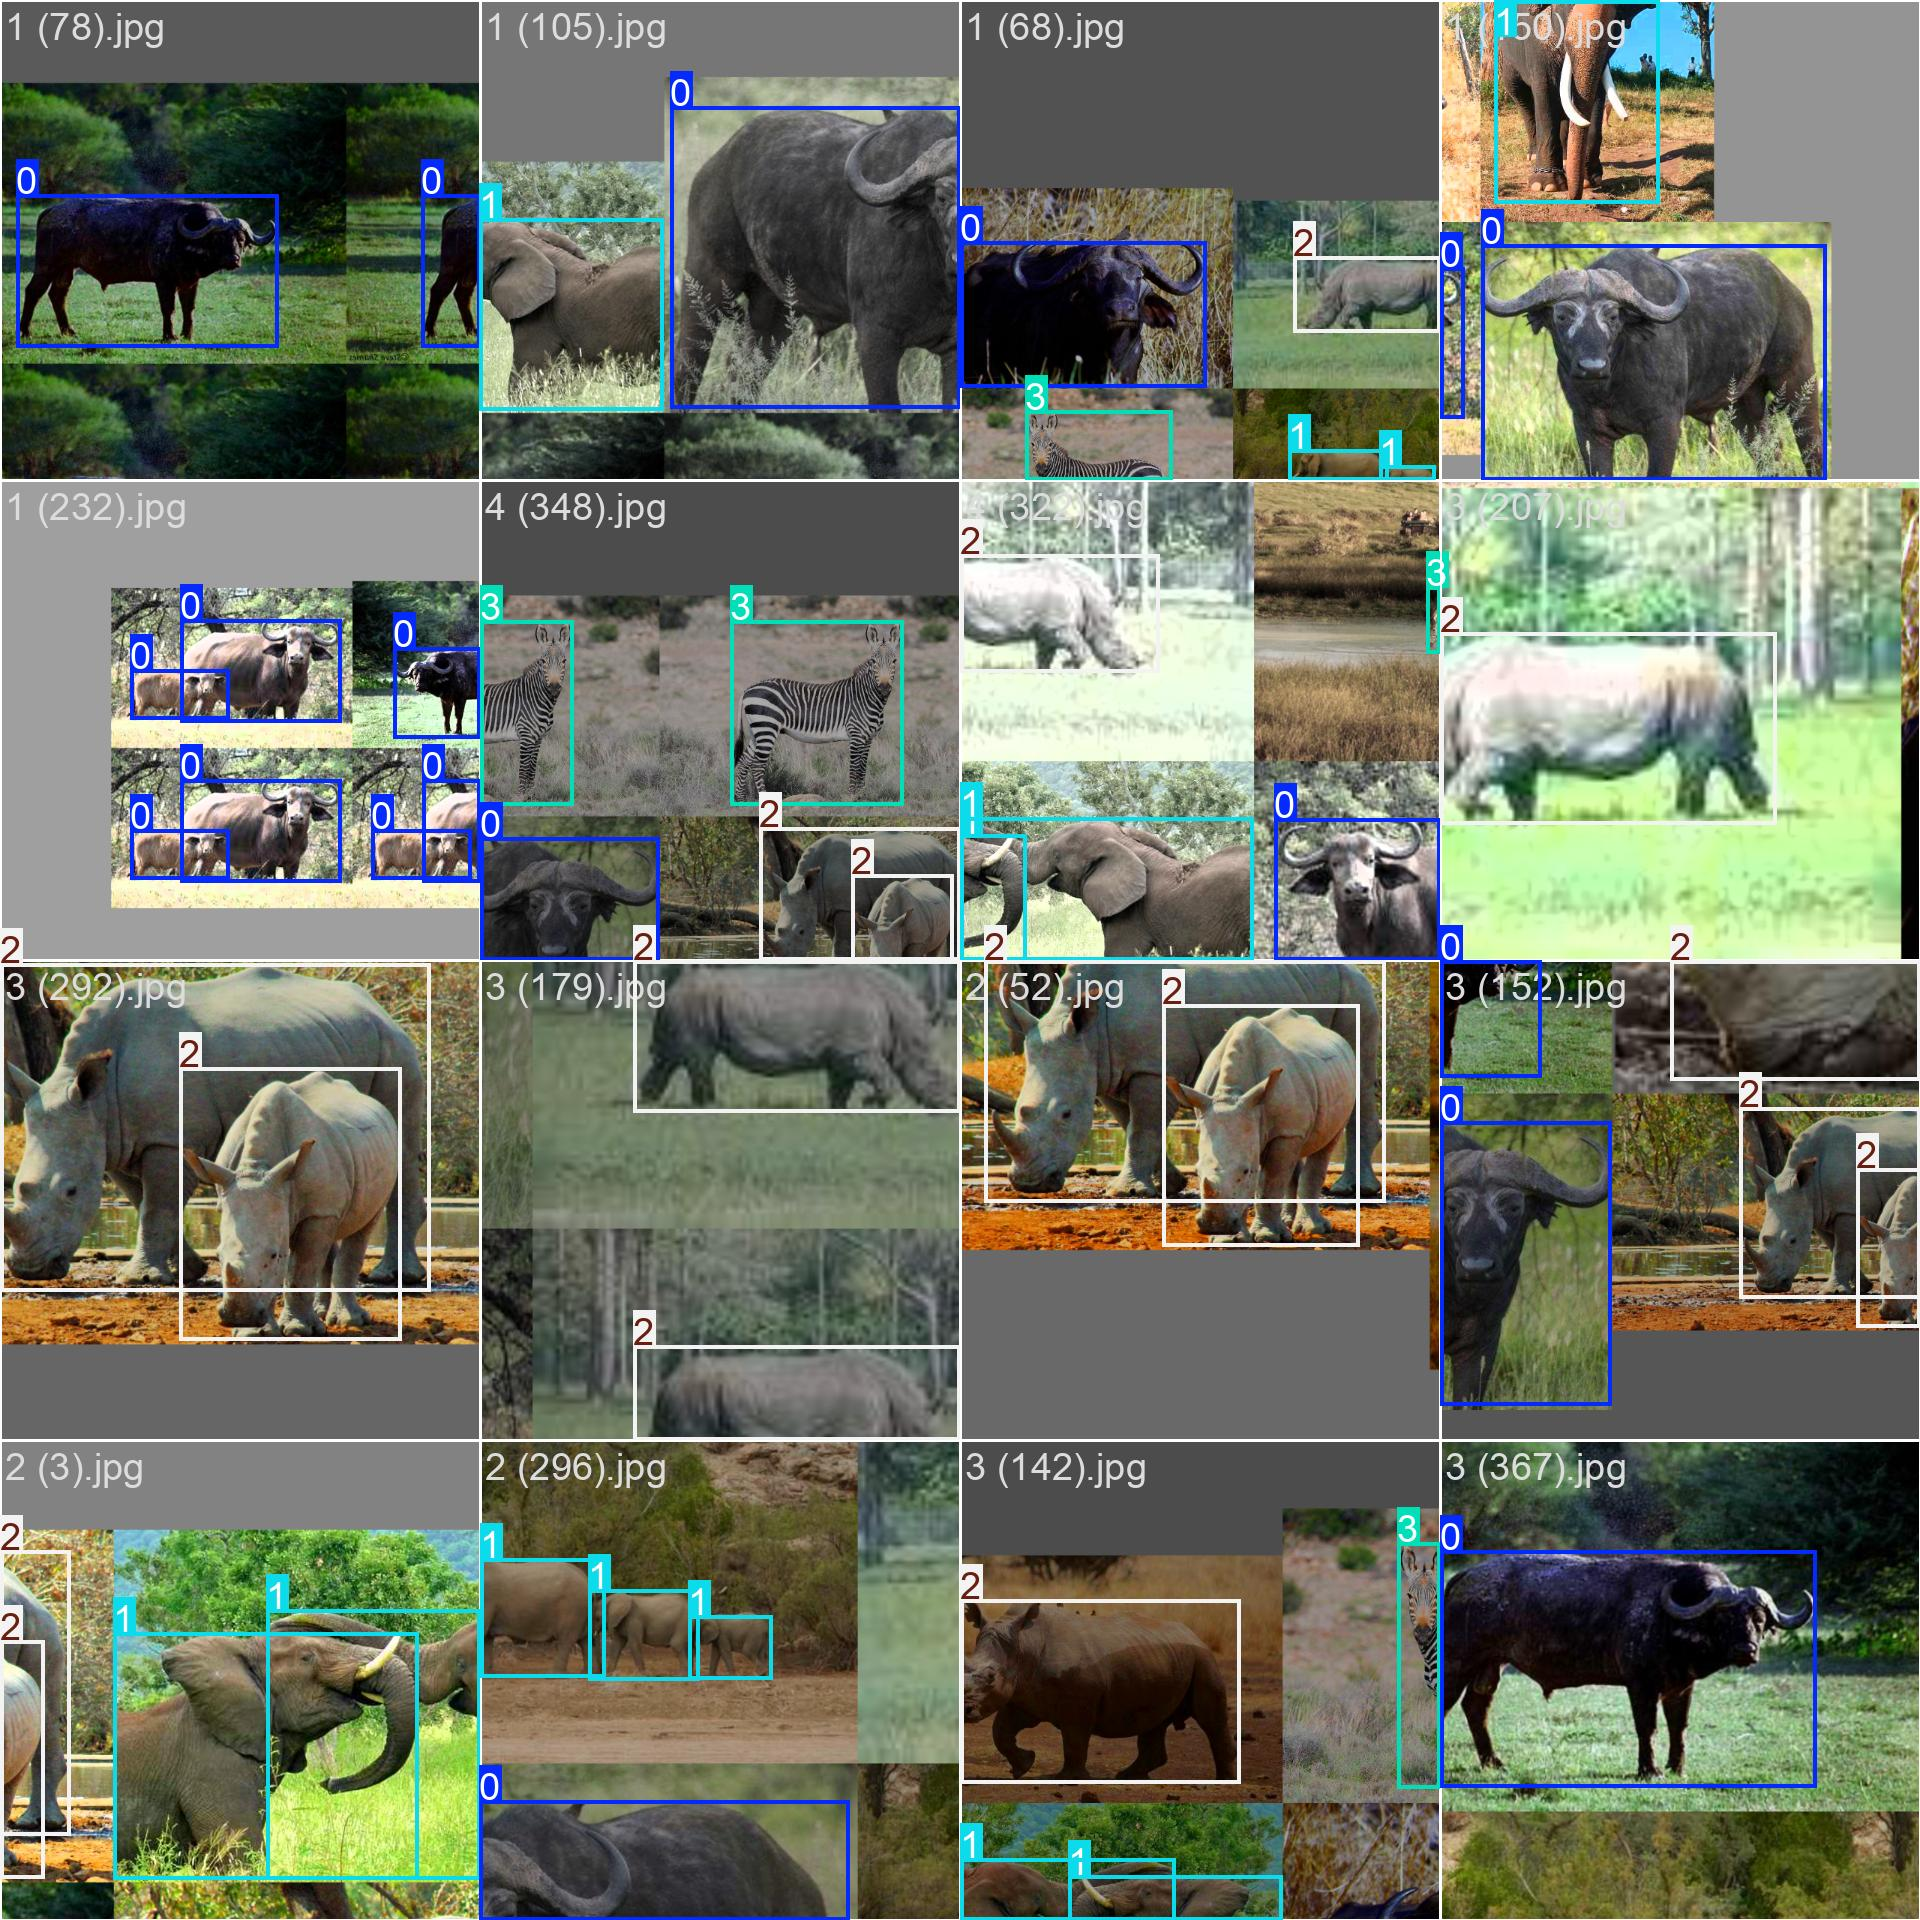
\includegraphics[width=0.52\textwidth]{train_batch.jpg}
\caption{Một lô ảnh huấn luyện do Ultralytics xuất ra. Có thể thấy phép tăng cường dữ liệu ghép
ảnh (mosaic) dán bốn ảnh gốc vào một khung: mô hình vì thế luôn nhìn thấy đối tượng ở nhiều tỉ lệ
và vị trí khác nhau, kể cả khi bộ dữ liệu nhỏ~\cite{bochkovskiy2020}.}
\label{fig:batch}
\end{figure}

\section{Phương pháp}

\subsection{Học chuyển giao thay vì huấn luyện từ đầu}

Với \ntrain{} ảnh huấn luyện thì huấn luyện một mạng phát hiện từ đầu là không khả thi --- số ảnh
này nhỏ hơn COCO khoảng hai bậc. Em dùng trọng số đã tiền huấn luyện trên COCO và huấn luyện tiếp
toàn bộ mạng trên dữ liệu mới. Lý do cách này hiệu quả đã được Yosinski và cộng sự phân tích từ
sớm~\cite{yosinski2014}: các tầng đầu của mạng tích chập học những thứ chung cho mọi ảnh tự nhiên
(cạnh, góc, kết cấu), nên gần như không phụ thuộc bài toán; càng về sau thì biểu diễn càng chuyên
biệt. Giữ lại phần chung đó và chỉ chỉnh phần chuyên biệt vừa nhanh hơn vừa ổn định hơn so với
khởi tạo ngẫu nhiên.

Riêng ở đây việc chuyển giao còn thuận lợi hơn bình thường, vì COCO đã có sẵn các lớp động vật
(voi, ngựa vằn, bò...). Mô hình không phải học khái niệm ``con vật bốn chân trong ảnh thiên nhiên''
từ con số không, mà chủ yếu học cách phân biệt bốn loài cụ thể.

\subsection{Mô hình dự đoán cái gì}

YOLO11 là mô hình không dùng hộp neo (anchor-free), tức mỗi vị trí trên bản đồ đặc trưng dự đoán
trực tiếp khoảng cách từ điểm đó tới bốn cạnh của hộp, thay vì tinh chỉnh một tập hộp mẫu định
trước như các phiên bản YOLO cũ; đây là hướng mà FCOS~\cite{tian2019} đề xuất.

Hàm mất mát có ba thành phần mà Ultralytics ghi riêng trong nhật ký huấn luyện, và em dùng tổng của
chúng để vẽ hình:

\begin{itemize}
  \item \texttt{cls\_loss} --- mất mát phân lớp, trả lời ``vật này thuộc lớp nào''.
  \item \texttt{box\_loss} --- mất mát định vị, đo độ khớp giữa hộp dự đoán và hộp thật.
  \item \texttt{dfl\_loss} --- Distribution Focal Loss~\cite{li2020}. Thay vì dự đoán mỗi cạnh hộp
        bằng một con số, mô hình dự đoán một phân phối rời rạc trên các vị trí khả dĩ của cạnh đó
        rồi lấy kỳ vọng. Cách này cho phép mạng biểu diễn được sự không chắc chắn khi biên của vật
        bị mờ hoặc bị che, điều mà một con số đơn lẻ không làm được.
\end{itemize}

\subsection{Giao thức huấn luyện và phần mã cấu hình}

Vì phép so sánh ba cỡ mô hình là nội dung chính, giao thức huấn luyện phải tuyệt đối giống nhau
giữa ba lần chạy. Để điều đó không phụ thuộc vào việc em có gõ đúng tham số hay không, em gom toàn
bộ giao thức vào một lớp dữ liệu duy nhất trong \texttt{src/yolo/config.py}; ba lần chạy gọi cùng
một đối tượng cấu hình và chỉ truyền vào ký hiệu cỡ mô hình.

\begin{lstlisting}
SIZES = ("n", "s", "m")
VERSION = "yolo11"

@dataclass(frozen=True)
class TrainConfig:
    """Everything that must be identical across the three model sizes."""
    task: str = "detect"
    epochs: int = 50
    imgsz: int = 416          # 640 khi chay tren GPU
    batch: int = 8            # 16 khi chay tren GPU
    seed: int = 42
    workers: int = 4
    device: str = "cpu"
    patience: int = 20
    optimizer: str = "auto"
    extra: dict = field(default_factory=dict)

    def train_args(self, size: str) -> dict:
        return {
            "data": self.data, "epochs": self.epochs, "imgsz": self.imgsz,
            "batch": self.batch, "seed": self.seed, "workers": self.workers,
            "device": self.device, "patience": self.patience,
            "optimizer": self.optimizer,
            "name": f"{VERSION}{size}", "exist_ok": True,
            "plots": True, "val": True, **self.extra,
        }
\end{lstlisting}

\begin{table}[H]
\centering
\caption{Giao thức huấn luyện. Ba cỡ mô hình dùng đúng các giá trị này; điểm khác duy nhất giữa ba lần chạy là tệp trọng số khởi tạo. Toàn bộ tham số được khai báo một chỗ trong \texttt{src/yolo/config.py} nên không thể lệch nhau giữa các lần chạy.}
\label{tab:protocol}
\small
\begin{tabular}{l l}
\toprule
Tham số & Giá trị \\
\midrule
Phiên bản mô hình & YOLO11 (yolo11n, yolo11s, yolo11m) \\
Trọng số khởi tạo & điểm kiểm tra tiền huấn luyện trên COCO của Ultralytics \\
Số epoch & 50 \\
Kích thước ảnh đầu vào & 640$\times$640 \\
Kích thước lô (batch) & 16 \\
Hạt giống ngẫu nhiên & 42 \\
Bộ tối ưu & tự động (\texttt{optimizer=auto}) theo Ultralytics \\
Tốc độ học & tăng tới 0{,}00119 sau 3 epoch khởi động, giảm dần còn $3{,}72\times 10^{-5}$ \\
Tăng cường dữ liệu & mặc định của Ultralytics; ghép ảnh (mosaic) tắt ở 10 epoch cuối \\
Kiên nhẫn dừng sớm & 20 epoch (không mô hình nào bị dừng sớm) \\
Phần cứng & GPU NVIDIA Tesla T4 trên Google Colab \\
\bottomrule
\end{tabular}
\end{table}


Lớp này được đánh dấu \texttt{frozen=True} nên không thể sửa giá trị sau khi tạo, và phương thức
\texttt{as\_record()} ghi toàn bộ tham số vào tệp kết quả cùng với các chỉ số --- nhờ vậy bảng kết
quả luôn mang theo điều kiện đã sinh ra nó. Vòng lặp huấn luyện trong \texttt{src/yolo/train.py}
chỉ làm ba việc: nạp điểm kiểm tra tương ứng với cỡ mô hình, gọi
\texttt{model.train(**config.train\_args(size))}, rồi chấm điểm mô hình trên phần \emph{test}
bằng \texttt{model.val(split="test")}. Em không cài lại bất kỳ phần nào của YOLO.

Một chi tiết em học được khi dựng phần này: Ultralytics lưu đường dẫn thư mục dữ liệu và thư mục
kết quả trong một tệp cấu hình \emph{toàn cục} của máy chứ không theo dự án, nên nếu không ghim lại
thì kết quả có thể rơi vào thư mục của một dự án khác. Trong sổ tay Colab em ghim hai đường dẫn này
ngay sau khi cài thư viện.

Ba mô hình được huấn luyện lần lượt trên GPU Tesla T4 của Google Colab, tổng cộng \totalminutes{}
phút. Trước đó em có đo thử trên CPU của máy cá nhân: một epoch của yolo11m ở \imgsz{} điểm ảnh mất
16,4 phút, tức riêng mô hình này đã cần hơn 13 giờ cho \epochs{} epoch. Phép đo đó là lý do em
chuyển sang Colab chứ không chạy ở máy.

\section{Kết quả}

Bảng~\ref{tab:results} là kết quả của ba mô hình trên phần \emph{test}, phần dữ liệu mà không mô
hình nào nhìn thấy trong lúc huấn luyện.

\begin{table}[H]
\centering
\caption{Kết quả trên tập giữ lại (test). Dòng cuối bảng là độ lệch chuẩn của mAP50-95 trong mười epoch cuối, đo trên tập val. Mức dao động lớn nhất (0{,}0141) lớn hơn khoảng cách giữa ba mô hình trên tập val (0{,}0080), nên thứ tự ba dòng trên không nên đọc như một bảng xếp hạng. Ký hiệu (B) chỉ chỉ số tính trên hộp giới hạn.}
\label{tab:results}
\small
\begin{tabular}{l r r r r r r}
\toprule
Mô hình & Tham số (M) & Thời gian (phút) & Precision & Recall & mAP50 & mAP50-95 \\
\midrule
yolo11n & 2{,}6 & 5{,}6 & 0{,}949 & 0{,}939 & 0{,}9713 & 0{,}8447 \\
yolo11s & 9{,}4 & 5{,}6 & 0{,}977 & 0{,}934 & 0{,}9772 & \textbf{0{,}8543} \\
yolo11m & 20{,}1 & 6{,}9 & 0{,}957 & 0{,}926 & 0{,}9693 & 0{,}8314 \\
\midrule
\multicolumn{7}{l}{\small Dao động mAP50-95 trên val, 10 epoch cuối: yolo11n 0{,}0083; yolo11s 0{,}0136; yolo11m 0{,}0141} \\
\bottomrule
\end{tabular}
\end{table}


Cả ba mô hình đều đạt mAP50 trên 0,96, nghĩa là với ngưỡng chồng lấn 0,5 thì gần như mọi con vật
trong ảnh đều được tìm thấy đúng lớp và đúng vị trí. Chỉ số khắt khe hơn là mAP50-95, lấy trung
bình độ chính xác qua mười ngưỡng chồng lấn từ 0,5 đến 0,95~\cite{everingham2010}: ở ngưỡng cao,
hộp dự đoán phải trùng gần như khít với hộp thật mới được tính là đúng. Con số này giảm xuống
khoảng 0,83--0,85, cho thấy phần sai còn lại chủ yếu không phải là ``không tìm thấy con vật'' mà là
``hộp chưa thật sát viền''.

\begin{figure}[H]
\centering
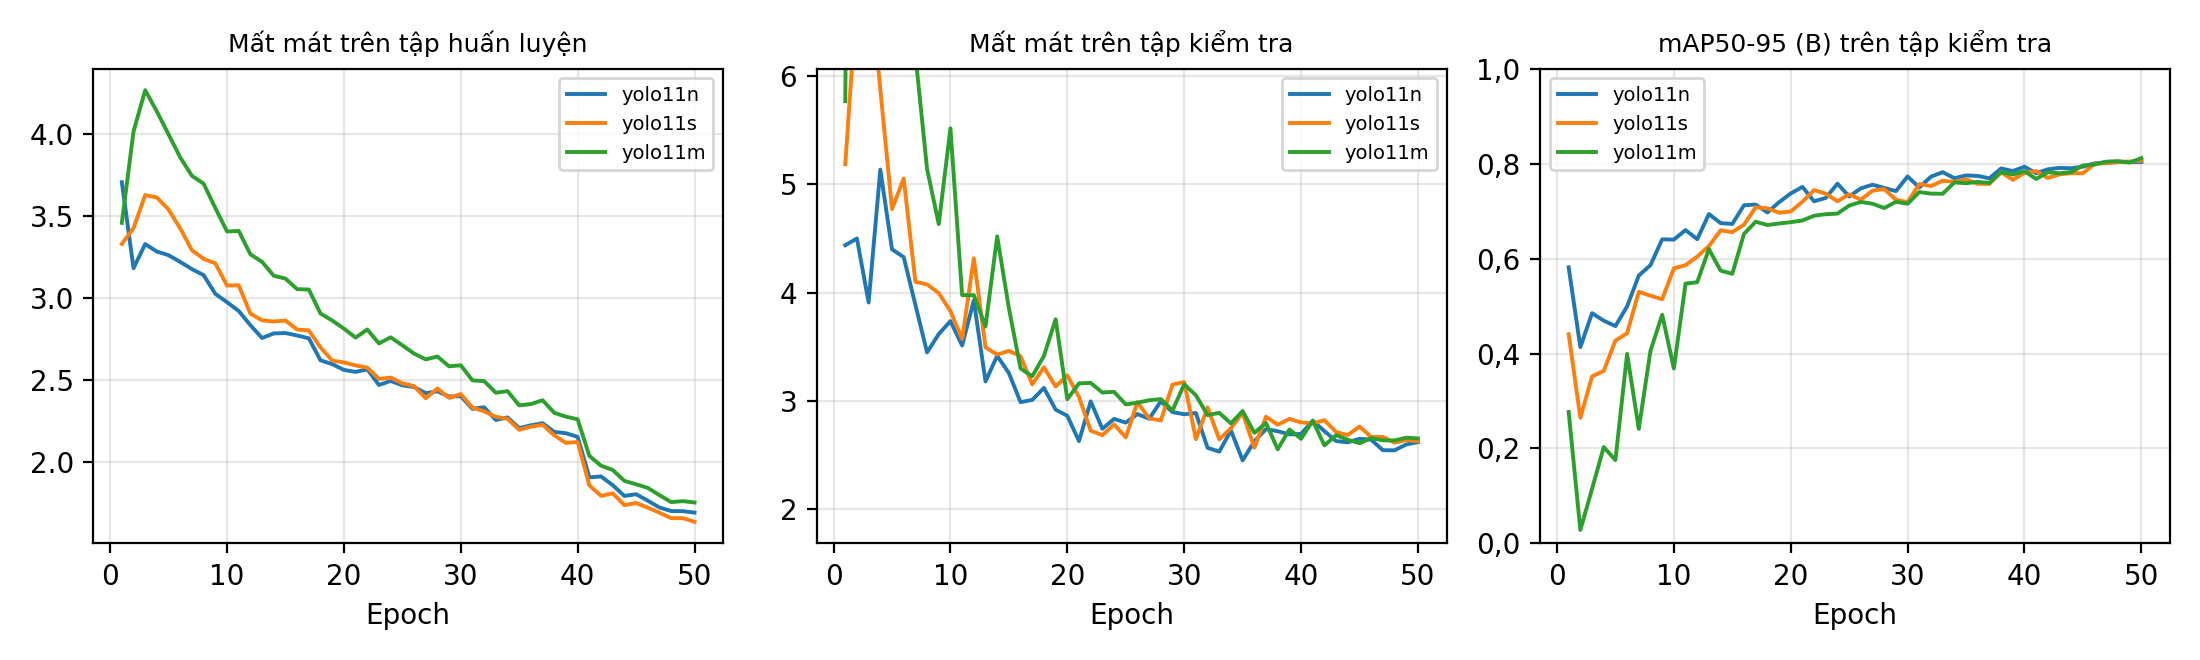
\includegraphics[width=\textwidth]{curves.png}
\caption{Mất mát và mAP theo từng epoch của ba mô hình, vẽ chung trục để so sánh được. Trục đứng
của ô giữa được cắt ngay trên mức mất mát từ epoch 8 trở đi, vì những epoch đầu của yolo11m vọt lên
rất cao và sẽ làm phẳng toàn bộ phần còn lại. Chỗ gãy tại epoch 40 ở ô bên trái là do Ultralytics
tắt phép ghép ảnh mosaic trong 10 epoch cuối, khiến dữ liệu huấn luyện đột ngột dễ hơn.}
\label{fig:curves}
\end{figure}

Hình~\ref{fig:curves} và Hình~\ref{fig:ultralytics} là bằng chứng huấn luyện mà đề bài yêu cầu;
Bảng~\ref{tab:log} bổ sung phần nhật ký thô do chính Ultralytics ghi ra sau mỗi epoch, để đối
chiếu được với các hình. Ba điều đọc được từ các đường cong:

\begin{itemize}
  \item Mất mát trên cả hai tập đều giảm đều và không tách nhau ở cuối, nên không có dấu hiệu quá
        khớp (overfitting) --- điều này hợp lý vì mô hình chỉ được huấn luyện \epochs{} epoch từ
        trọng số đã tốt sẵn.
  \item Mô hình lớn nhất khởi đầu \emph{tệ nhất}: trong mười epoch đầu, mAP của yolo11m thấp hơn
        hẳn hai mô hình kia và mất mát trên tập val của nó vọt lên rất cao. Nhiều tham số hơn nghĩa
        là cần nhiều bước hơn để ổn định, chứ không phải tốt hơn ngay.
  \item Từ khoảng epoch 25 trở đi, ba đường gần như chồng lên nhau. Đây là quan sát dẫn tới phần
        phân tích bên dưới.
\end{itemize}

\begin{table}[H]
\centering
\caption{Trích nhật ký huấn luyện của yolo11n, chép trực tiếp từ \texttt{runs/detect/yolo11n/results.csv} --- tệp do Ultralytics ghi sau mỗi epoch trong lúc chạy. Cột thời gian là giây tính từ lúc bắt đầu.}
\label{tab:log}
\small
\begin{tabular}{r r r r r r}
\toprule
Epoch & Thời gian (s) & Mất mát HL & Mất mát KT & mAP50 (B) & mAP50-95 (B) \\
\midrule
1 & 14{,}4 & 3{,}706 & 4{,}437 & 0{,}8480 & 0{,}5814 \\
2 & 20{,}6 & 3{,}183 & 4{,}499 & 0{,}6002 & 0{,}4133 \\
3 & 26{,}8 & 3{,}329 & 3{,}908 & 0{,}7079 & 0{,}4850 \\
\multicolumn{6}{c}{\dots} \\
49 & 306{,}0 & 1{,}704 & 2{,}599 & 0{,}9555 & 0{,}8031 \\
50 & 311{,}9 & 1{,}695 & 2{,}621 & 0{,}9557 & 0{,}8034 \\
\bottomrule
\end{tabular}
\end{table}


\begin{figure}[H]
\centering
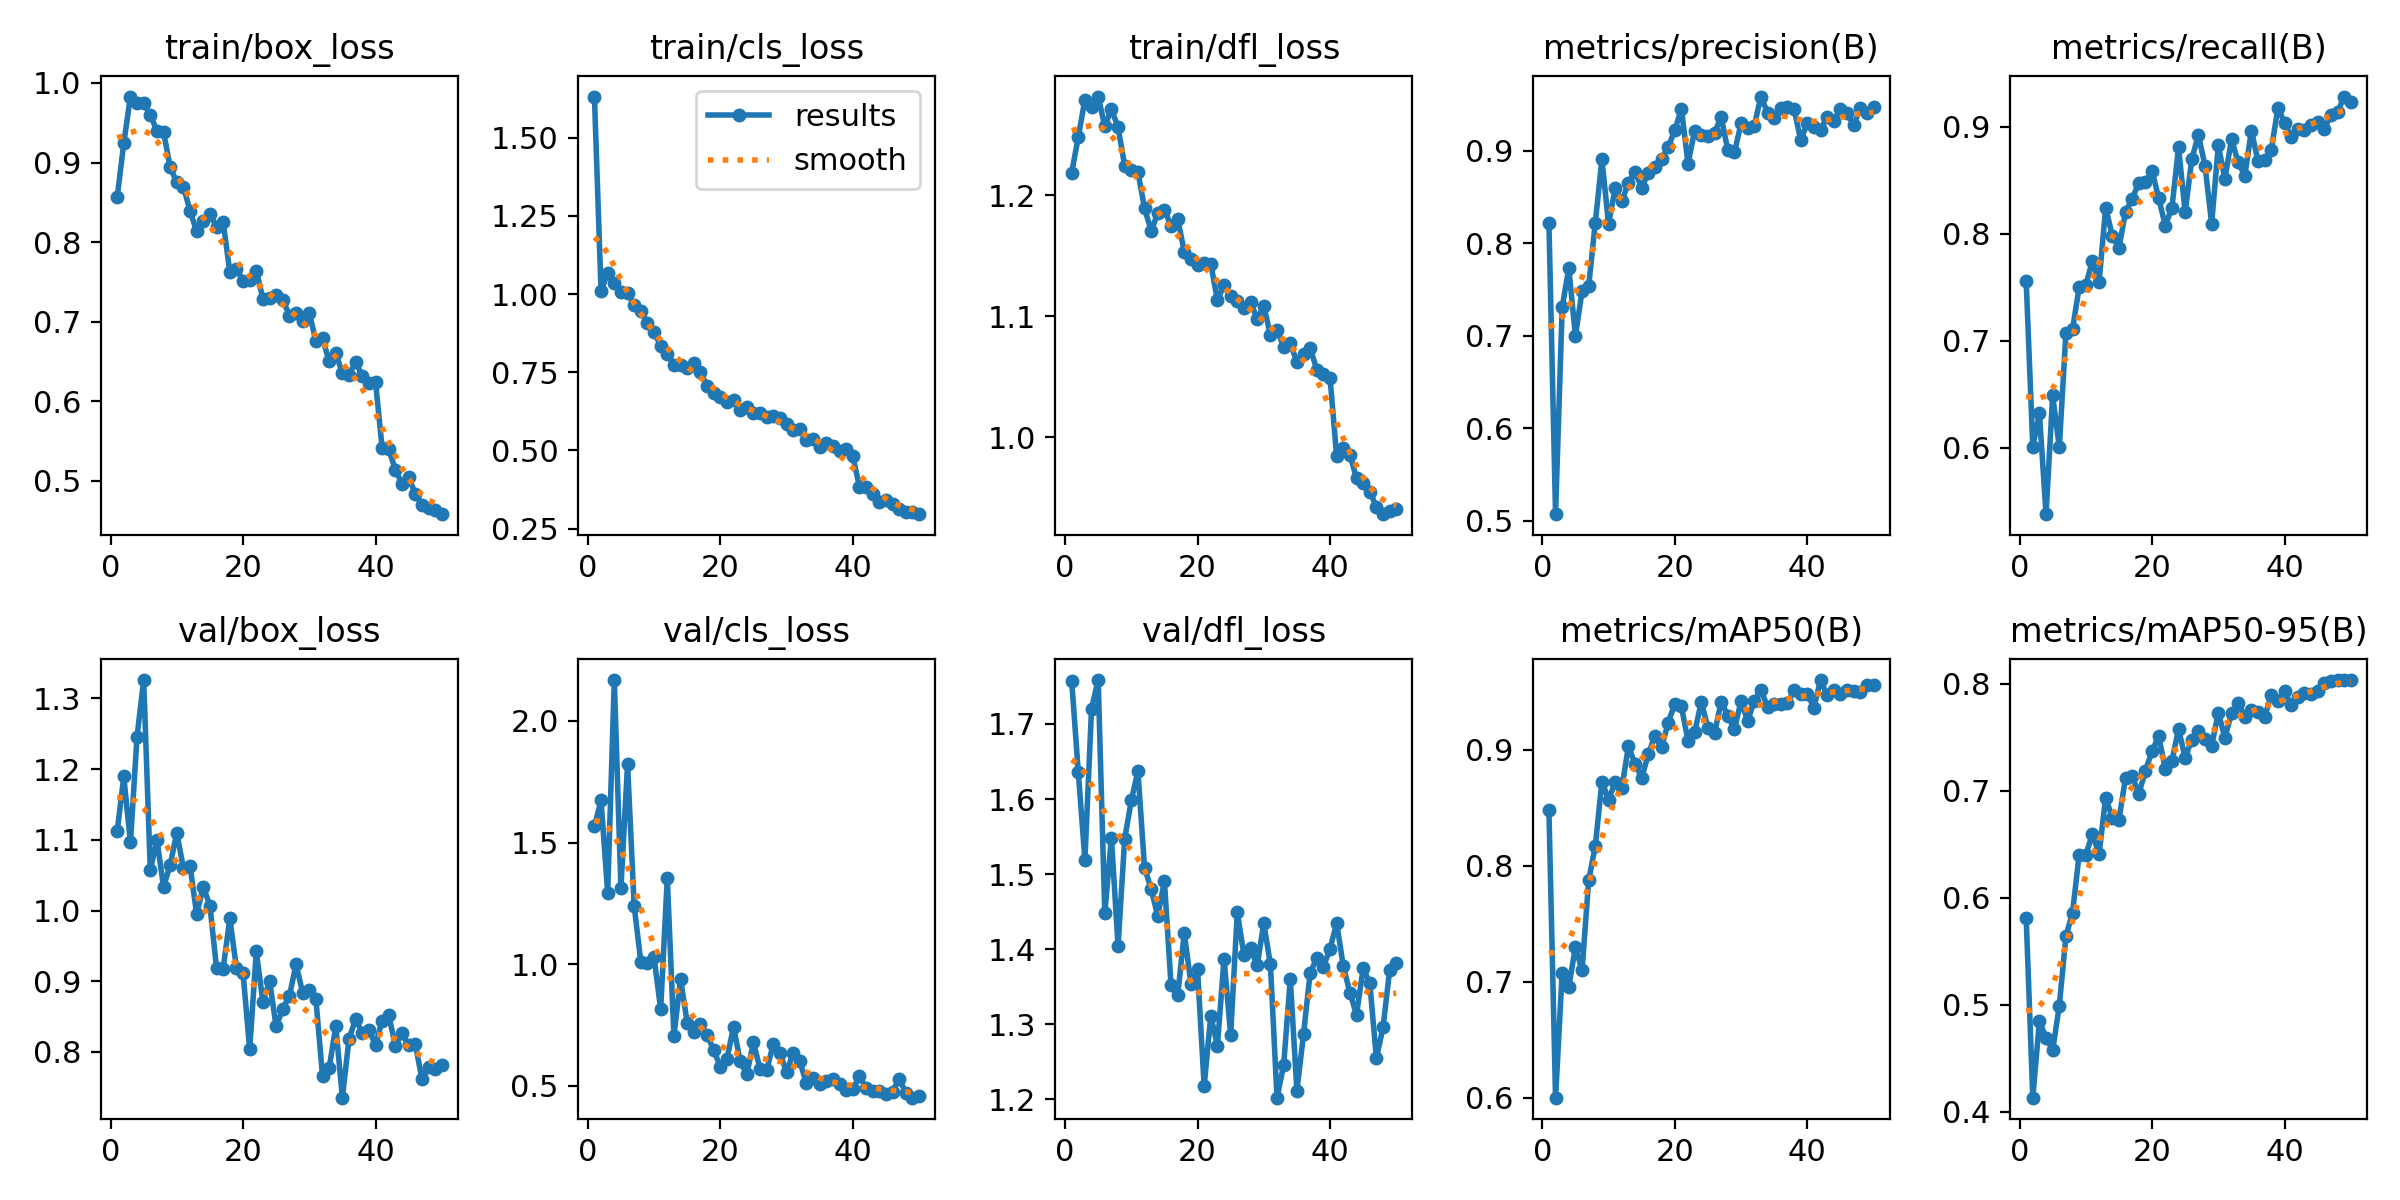
\includegraphics[width=0.78\textwidth]{ultralytics_n.png}
\caption{Toàn bộ nhật ký huấn luyện của yolo11n do Ultralytics tự xuất ra
(\texttt{runs/detect/yolo11n/results.png}): ba thành phần mất mát trên tập huấn luyện và tập kiểm
tra, cùng precision, recall, mAP50 và mAP50-95 theo epoch.}
\label{fig:ultralytics}
\end{figure}

\begin{figure}[H]
\centering
\begin{minipage}{0.48\textwidth}
  \centering
  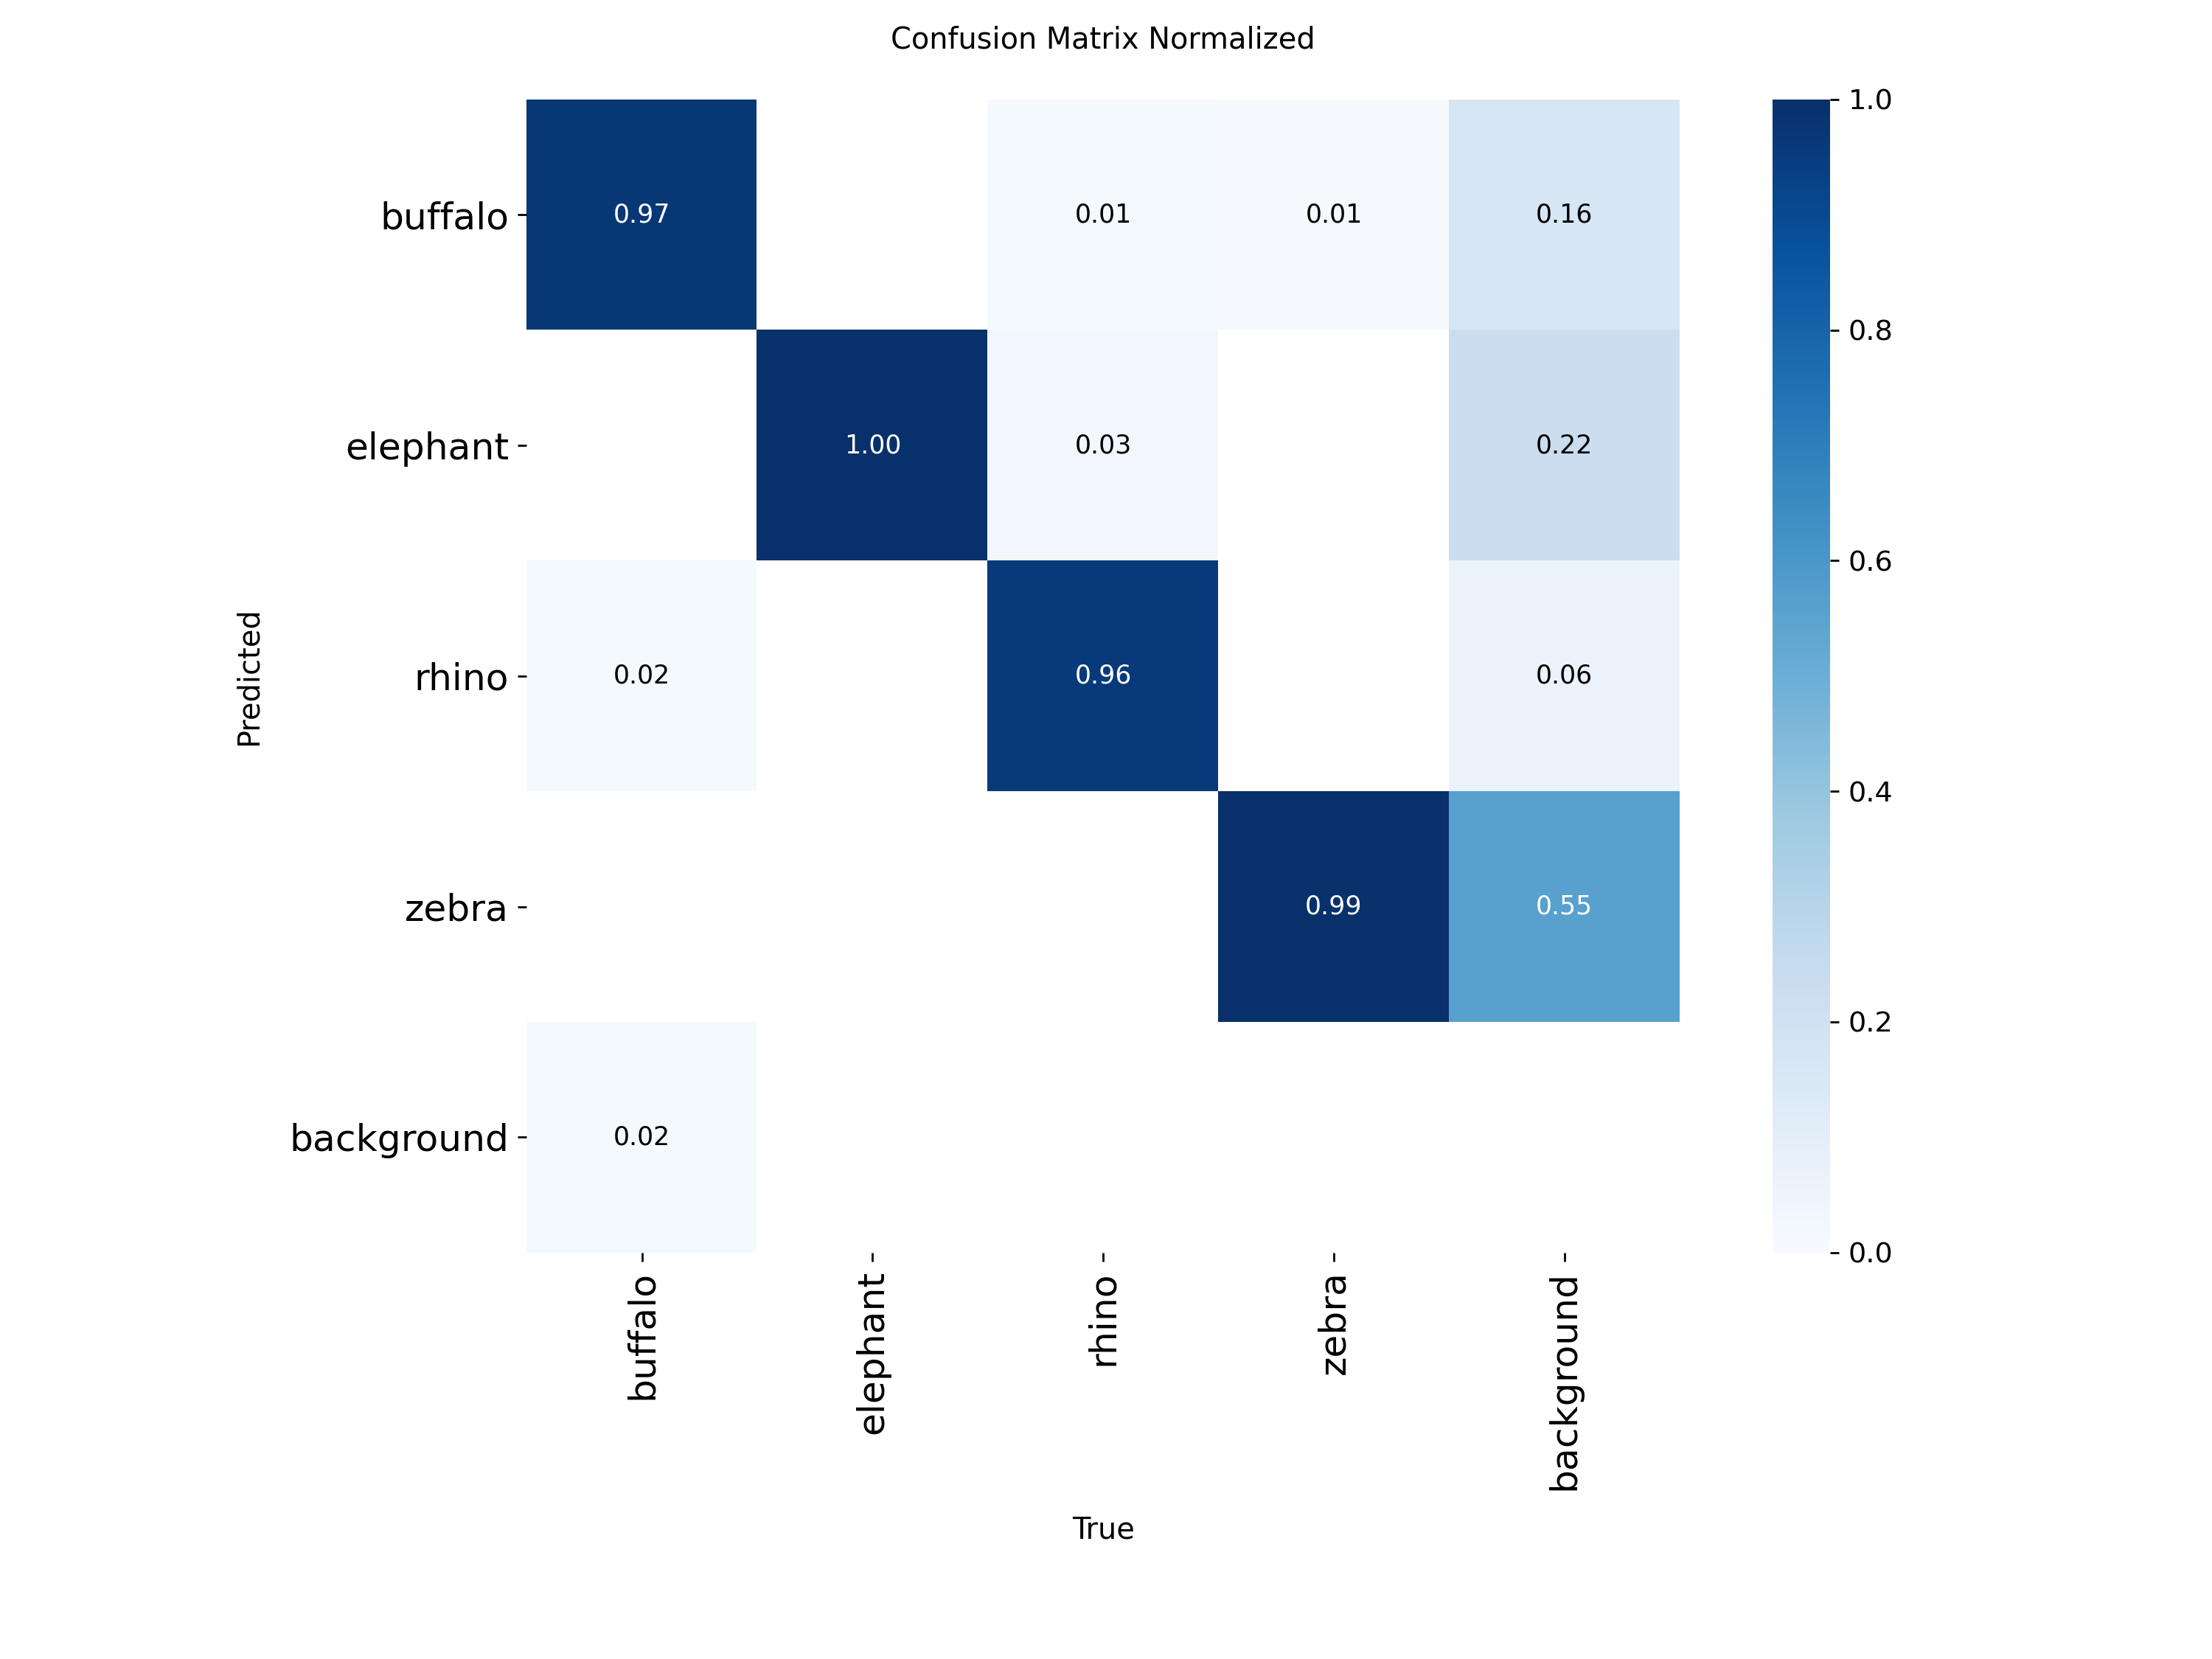
\includegraphics[width=\textwidth]{confusion.png}
\end{minipage}\hfill
\begin{minipage}{0.48\textwidth}
  \centering
  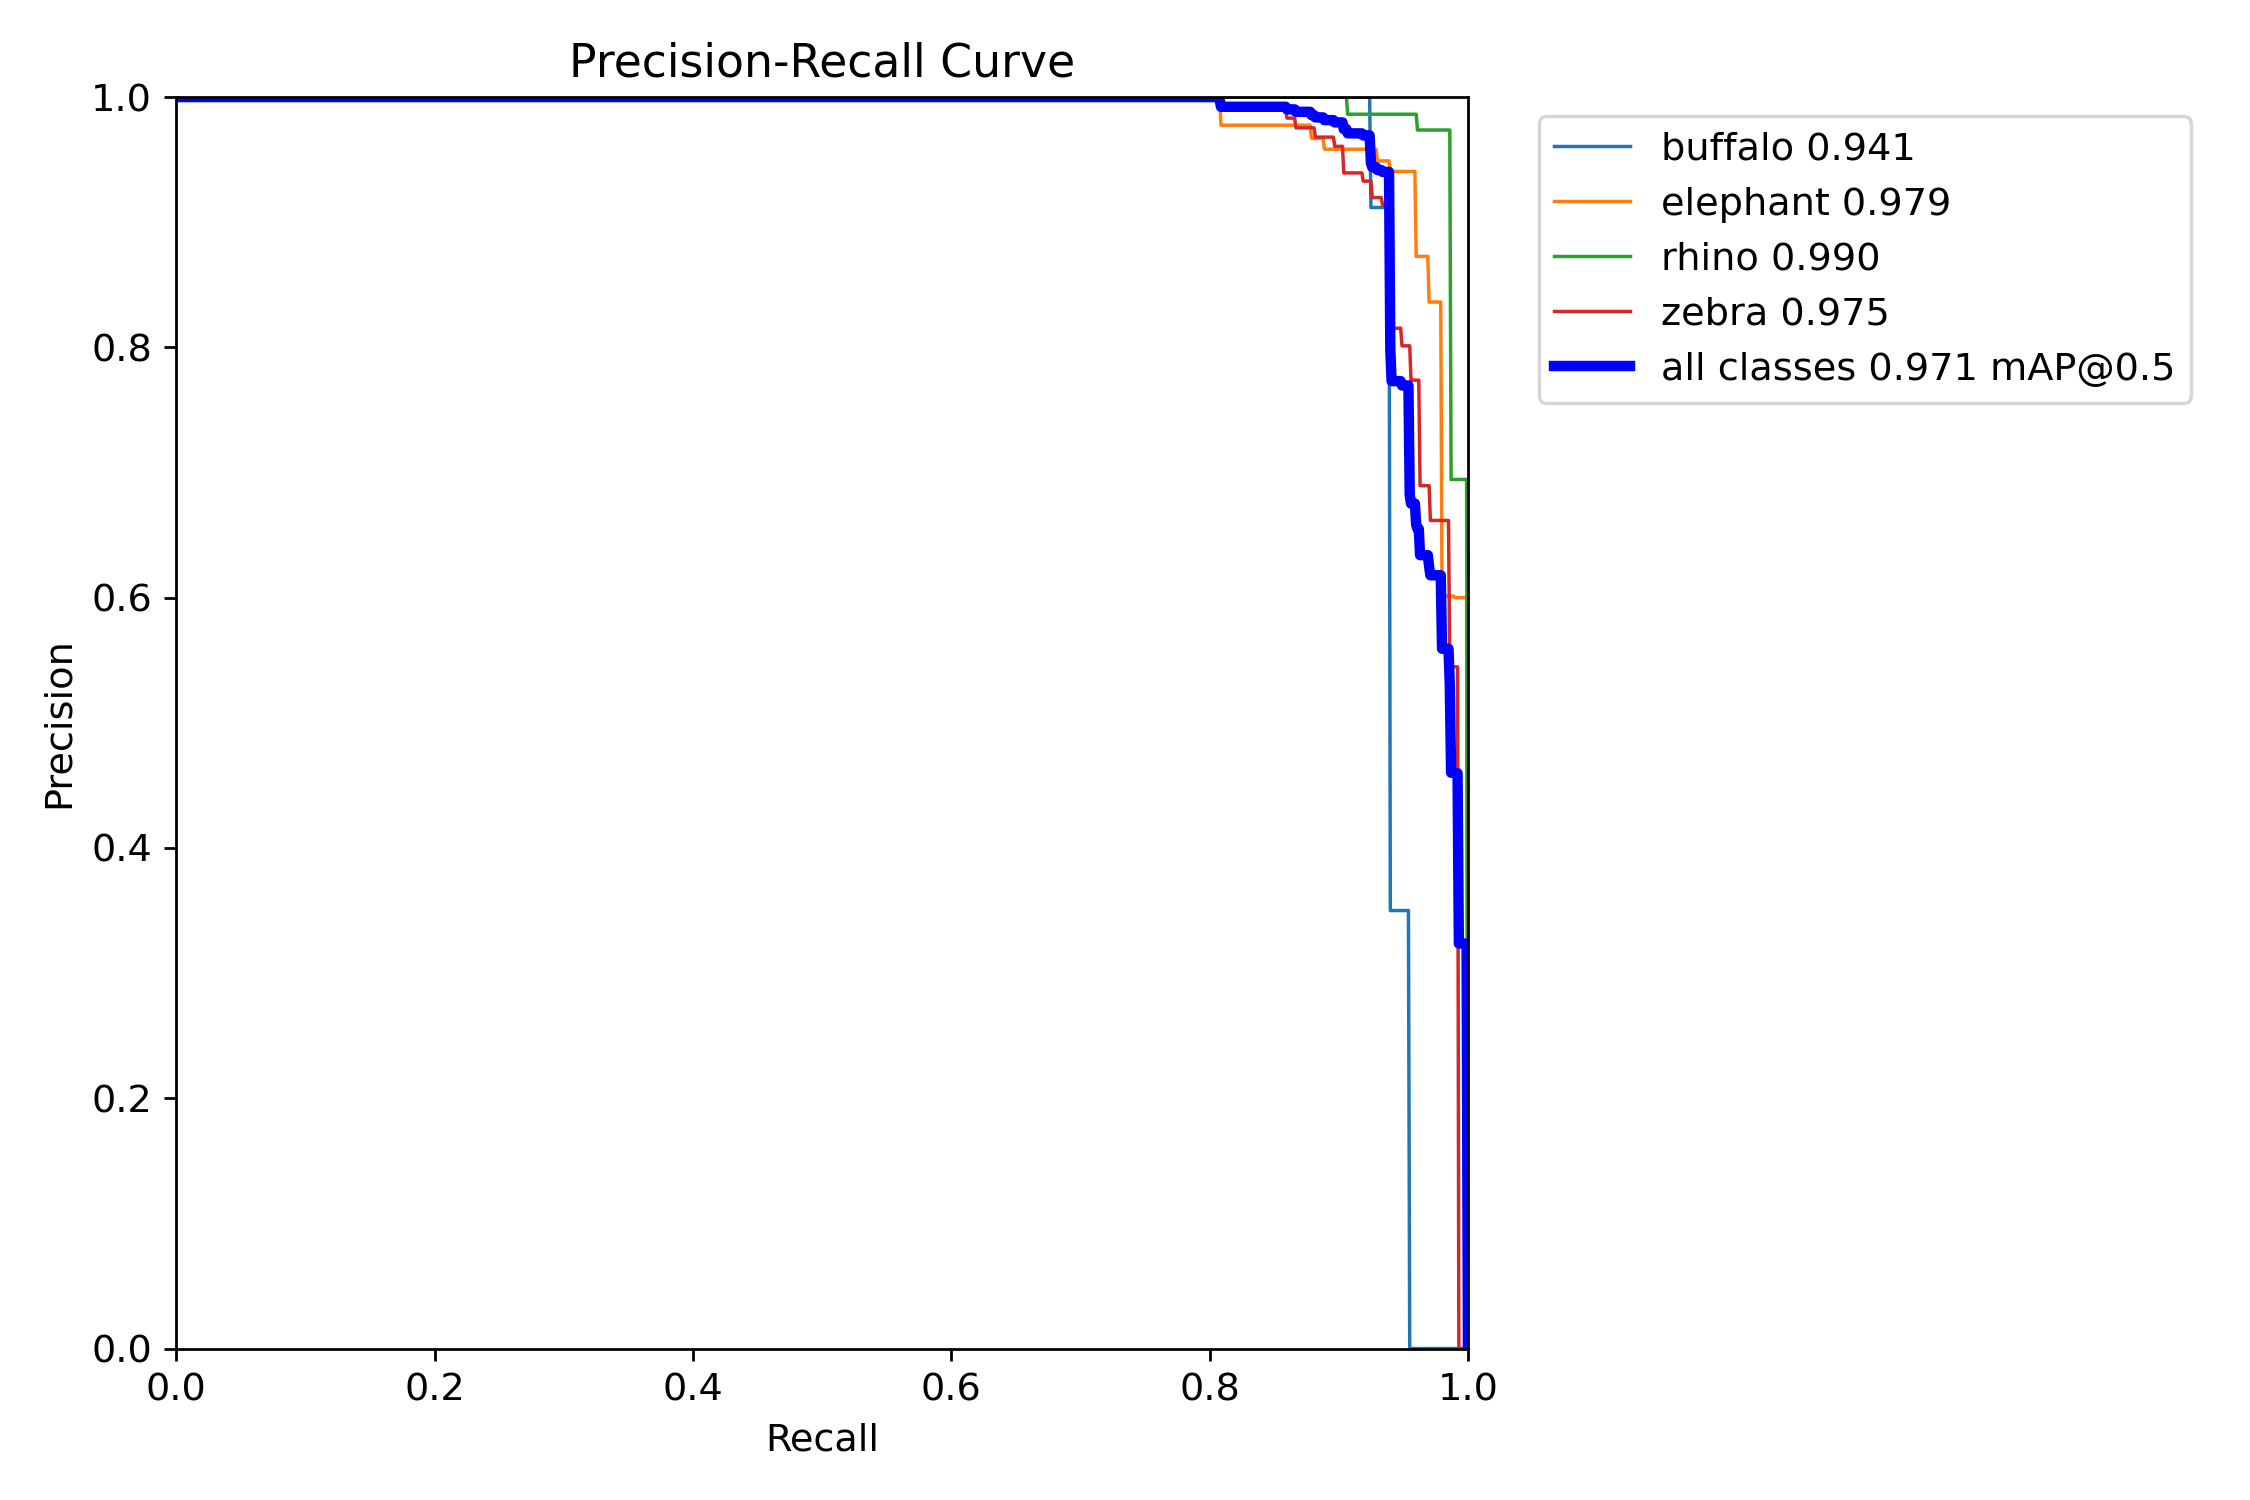
\includegraphics[width=\textwidth]{pr_curve.png}
\end{minipage}
\caption{Trái: ma trận nhầm lẫn chuẩn hoá của yolo11n trên phần test. Phải: đường
precision--recall của cùng mô hình. Cột và hàng \emph{background} là phần đáng chú ý: lỗi chủ yếu
không phải nhầm loài này với loài kia mà là bỏ sót con vật hoặc báo nhầm một vùng nền thành con
vật.}
\label{fig:confusion}
\end{figure}

Ma trận nhầm lẫn ở Hình~\ref{fig:confusion} cho thấy bốn loài gần như không bị nhầm lẫn với nhau.
Điều này khác hẳn bài tập phân lớp lá cây, nơi các loài giống nhau về hình dạng thường bị đổi chỗ
cho nhau. Ở đây bốn loài khác nhau rõ về màu sắc và dáng, nên phần khó của bài toán nằm ở khâu
định vị chứ không phải khâu phân biệt lớp.

\begin{figure}[H]
\centering
\begin{minipage}{0.48\textwidth}
  \centering
  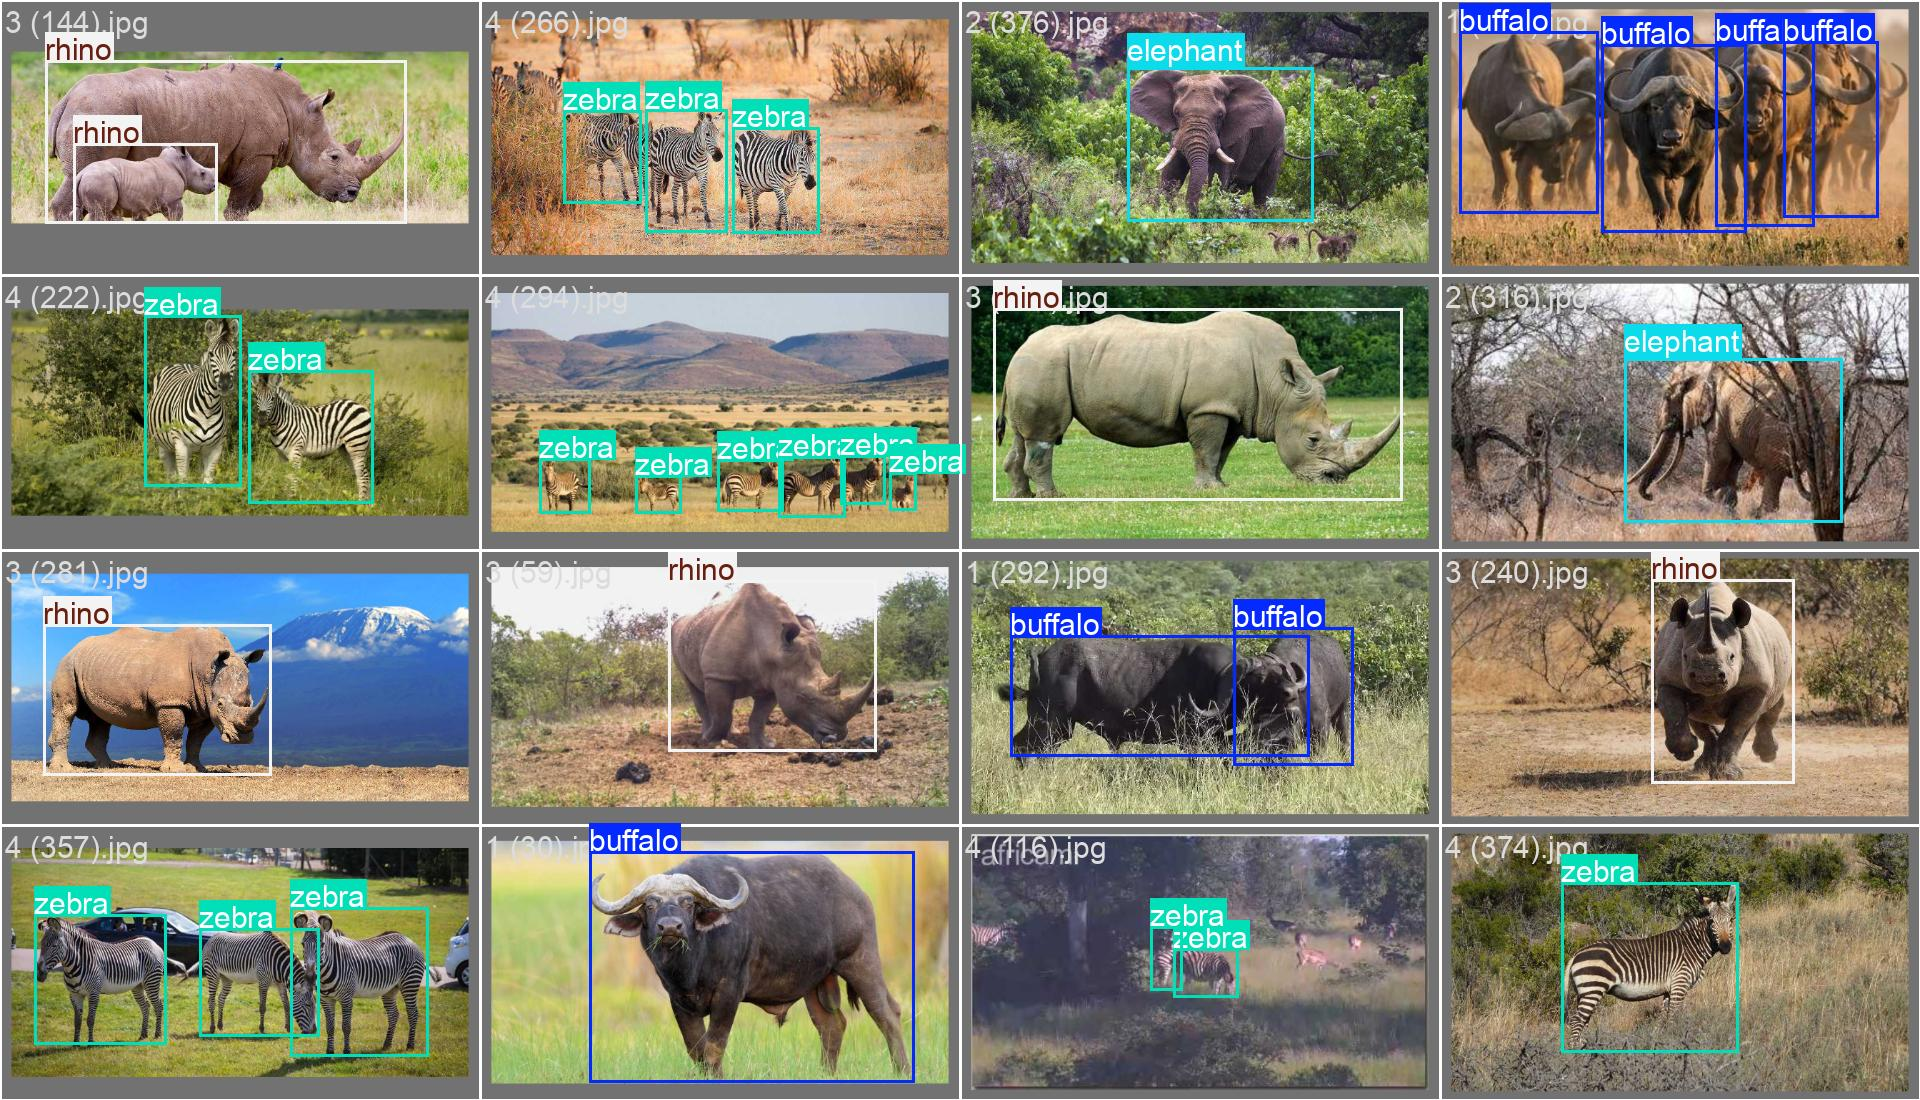
\includegraphics[width=\textwidth]{ground_truth.jpg}\\ {\small Nhãn thật}
\end{minipage}\hfill
\begin{minipage}{0.48\textwidth}
  \centering
  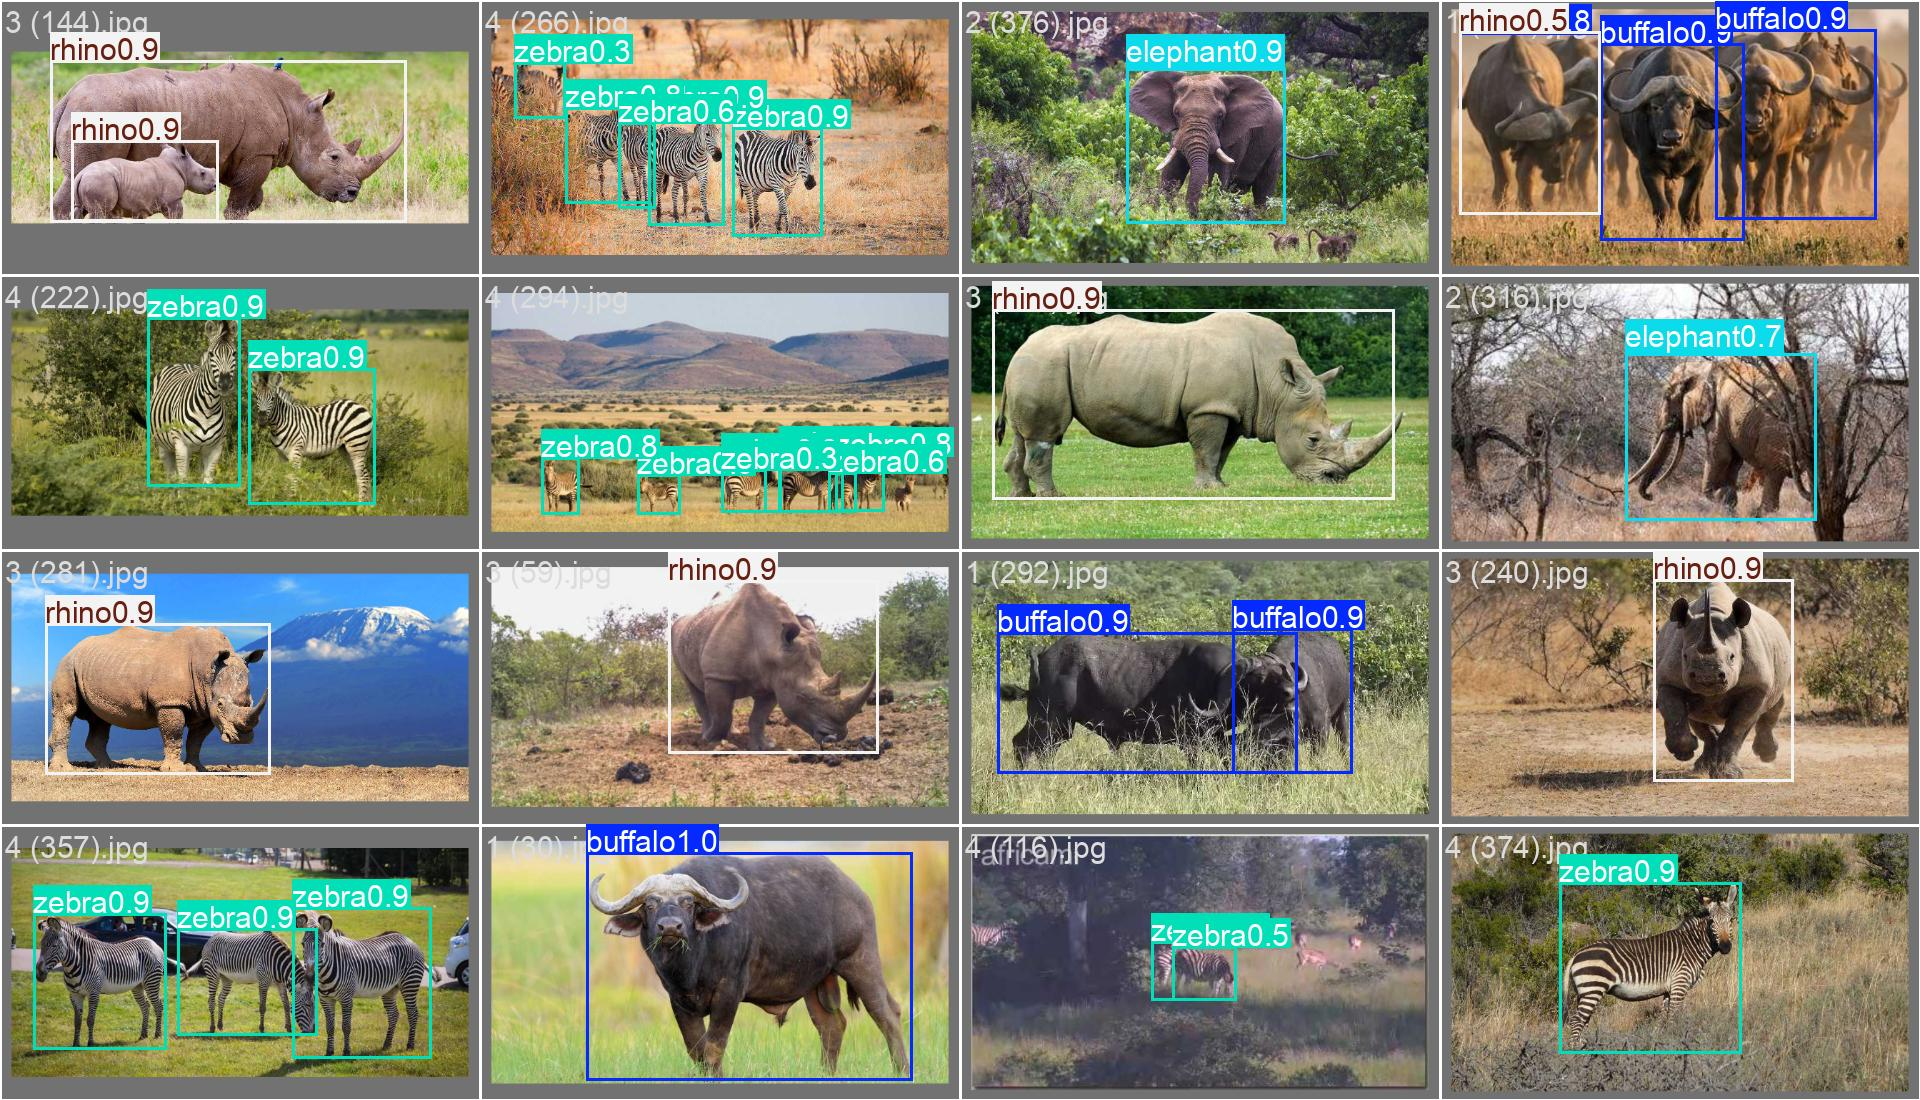
\includegraphics[width=\textwidth]{predictions.jpg}\\ {\small Dự đoán của yolo11n}
\end{minipage}
\caption{Một lô ảnh trong phần test: nhãn do người gán (trái) và dự đoán của mô hình nhẹ nhất
(phải), kèm điểm tin cậy. Các trường hợp còn sai thường rơi vào ảnh có nhiều con vật đứng chồng
lên nhau ở xa.}
\label{fig:predictions}
\end{figure}

\section{Phân tích: ba cỡ mô hình có thật sự khác nhau không?}

Nhìn Bảng~\ref{tab:results}, phản xạ tự nhiên là kết luận ``\besttest{} tốt nhất''. Em cho rằng
kết luận đó không đứng vững, vì hai lý do.

\textbf{Thứ nhất, khoảng cách giữa ba mô hình nhỏ hơn mức dao động của chính chúng.} Trong mười
epoch cuối, khi cả ba mô hình đã hội tụ và chỉ còn dao động quanh một mức, độ lệch chuẩn của
mAP50-95 là \nstd{} (yolo11n), \sstd{} (yolo11s) và \mstd{} (yolo11m). Trong khi đó khoảng cách
giữa mô hình cao nhất và thấp nhất chỉ là \valspread{} trên tập val. Nói cách khác, chỉ cần dừng
huấn luyện sớm hoặc muộn một epoch là đủ để đổi thứ tự xếp hạng. Đây đúng là bài học em đã gặp ở
bài tập 2, nơi kiểm định t theo cặp cho thấy phần lớn chênh lệch giữa các kiến trúc là nhiễu.

\begin{table}[H]
\centering
\caption{Cùng một chỉ số, đo trên hai tập dữ liệu khác nhau. Hai cột cho hai thứ tự xếp hạng khác nhau, trong khi cả hai khoảng cách đều nhỏ hơn mức dao động của chính mỗi mô hình giữa các epoch.}
\label{tab:ordering}
\small
\begin{tabular}{l r r}
\toprule
Mô hình & mAP50-95 trên val & mAP50-95 trên test \\
\midrule
yolo11n & 0{,}8034 & 0{,}8447 \\
yolo11s & 0{,}8061 & 0{,}8543 \\
yolo11m & 0{,}8114 & 0{,}8314 \\
\midrule
Khoảng cách lớn nhất--nhỏ nhất & 0{,}0080 & 0{,}0229 \\
\bottomrule
\end{tabular}
\end{table}


\textbf{Thứ hai, thứ tự xếp hạng đảo chiều khi đổi tập đánh giá.} Bảng~\ref{tab:ordering} đặt cạnh
nhau cùng một chỉ số đo trên hai tập dữ liệu khác nhau. Trên tập val, thứ tự đúng như kỳ vọng:
mô hình càng lớn càng tốt, và \bestval{} đứng đầu. Trên phần test thì \worsttest{} lại xuống thấp
nhất. Hai tập này có kích thước gần bằng nhau (\nval{} và \ntest{} ảnh) và cùng lấy từ một nguồn,
nên không có lý do nào để tin tập này ``đúng'' hơn tập kia. Cách đọc hợp lý là cả hai thứ tự đều
không mang thông tin.

\begin{figure}[H]
\centering
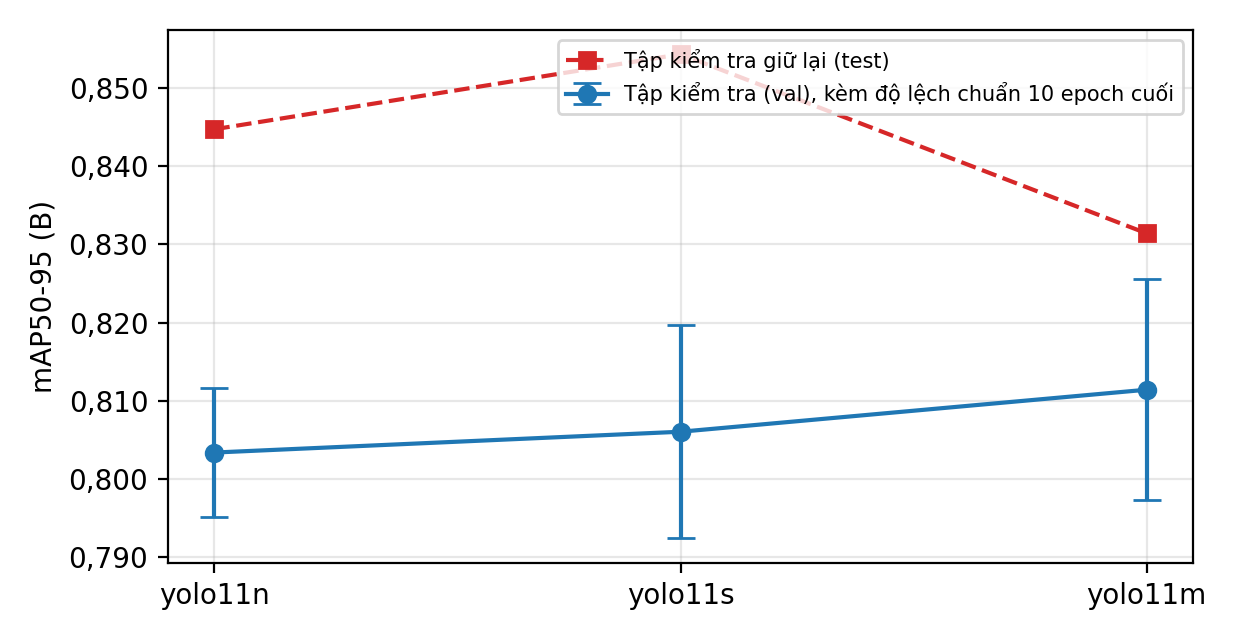
\includegraphics[width=0.74\textwidth]{val_vs_test.png}
\caption{mAP50-95 của ba mô hình trên hai tập đánh giá. Thanh sai số là độ lệch chuẩn của chính mô
hình đó trong mười epoch cuối. Các thanh sai số phủ lên nhau hoàn toàn, và hai đường không cùng
chiều --- hai dấu hiệu cho thấy không nên xếp hạng ba mô hình theo các con số này.}
\label{fig:gap}
\end{figure}

Vậy kết luận đúng là gì? Em cho rằng nó nằm ở chỗ khác: \textbf{năng lực của mô hình nhỏ nhất đã
dư cho bài toán này}. Với \nclasses{} lớp phân biệt rõ ràng, \objperimage{} đối tượng mỗi ảnh và
đối tượng chiếm diện tích lớn trong khung hình, phần khó không nằm ở sức biểu diễn của mạng. Tăng
số tham số từ \nparams{} triệu lên \mparams{} triệu --- gấp \paramratio{} lần --- không đổi được
điều đó. Trong tình huống này, chọn yolo11n là hợp lý: nó cho độ chính xác tương đương, nhẹ hơn
nhiều khi triển khai, và chạy nhanh hơn khi suy luận.

\textbf{Về thời gian huấn luyện}, có một điểm em muốn nói rõ để tránh hiểu nhầm. Mô hình m chỉ chậm
hơn mô hình n \timeratio{} lần (\mminutes{} phút so với \nminutes{} phút), trong khi nó nặng gấp
\paramratio{} lần về tham số. Tỉ lệ này không phản ánh chi phí tính toán thật của mô hình: với một
bộ dữ liệu nhỏ như thế này trên GPU T4, phần lớn thời gian mỗi epoch dành cho việc đọc và tăng
cường ảnh chứ không phải cho phép nhân ma trận. Muốn so sánh chi phí của ba mô hình thì phải đo
thời gian suy luận trên cùng một lô ảnh, không thể suy ra từ cột thời gian huấn luyện.

\section{Hạn chế}

Em nêu ba hạn chế mà bản thân kết quả không che được.

\textbf{Số epoch còn ngắn.} Cả ba mô hình đều đạt mAP cao nhất trên tập val đúng ở epoch cuối
(epoch \nbestepoch{}, \sbestepoch{} và \mbestepoch{}), tức đường cong vẫn đang đi lên khi huấn
luyện dừng. Cơ chế dừng sớm với \patience{} epoch kiên nhẫn không hề kích hoạt. Nếu chạy 100 hoặc
150 epoch, rất có thể mô hình lớn sẽ tách khỏi hai mô hình kia --- kết luận ``ba mô hình như nhau''
của báo cáo này chỉ đúng trong điều kiện \epochs{} epoch.

\textbf{Mỗi cấu hình chỉ chạy một lần.} Em ước lượng nhiễu bằng dao động giữa các epoch ở cuối quá
trình huấn luyện, đây là cách xấp xỉ. Cách chặt chẽ hơn là chạy lại mỗi mô hình với vài hạt giống
ngẫu nhiên khác nhau rồi so sánh phân bố, như kiểu kiểm định theo cặp em dùng ở hai bài trước.
Với ba mô hình và ba hạt giống thì chi phí gấp ba, vẫn nằm trong khả năng của Colab, và đây là việc
em sẽ làm nếu có thêm thời gian.

\textbf{Bộ dữ liệu dễ.} Đối tượng lớn, nền tương đối đơn giản, bốn lớp khác nhau rõ. Kết luận
``mô hình nhỏ là đủ'' gắn với đặc điểm này của dữ liệu, không nên đem áp cho bài toán có nhiều đối
tượng nhỏ hoặc nhiều lớp dễ nhầm.

\section{Kết luận}

Em đã huấn luyện ba cỡ mô hình YOLO11 trên bộ \dataname{} theo đúng một giao thức, bằng học chuyển
giao từ trọng số COCO, và chấm điểm trên phần dữ liệu giữ lại. Kết quả cao nhất là mAP50-95
\besttestmap{} của \besttest{}, với mAP50 của cả ba mô hình đều trên 0,96.

Điều em rút ra không nằm ở con số cao nhất. Ba cỡ mô hình chênh nhau \paramratio{} lần về số tham
số nhưng chênh nhau chưa tới \testspread{} điểm mAP, nhỏ hơn mức dao động giữa các epoch của chính
chúng, và thứ tự xếp hạng còn đảo chiều khi đổi tập đánh giá. Vì vậy báo cáo không khẳng định mô
hình nào tốt hơn mô hình nào, mà kết luận rằng với bài toán cỡ này, mô hình nhỏ nhất đã đủ --- và
rằng một bảng so sánh chỉ đáng tin khi khoảng cách giữa các dòng lớn hơn nhiễu của phép đo.

\begin{thebibliography}{9}

\bibitem{redmon2016}
J. Redmon, S. Divvala, R. Girshick, and A. Farhadi,
``You Only Look Once: Unified, Real-Time Object Detection,''
in \emph{Proc. IEEE Conf. Computer Vision and Pattern Recognition (CVPR)}, 2016, pp. 779--788.

\bibitem{khanam2024}
R. Khanam and M. Hussain,
``YOLOv11: An Overview of the Key Architectural Enhancements,''
arXiv preprint arXiv:2410.17725, 2024.

\bibitem{jocher2023}
G. Jocher, J. Qiu, and A. Chaurasia,
``Ultralytics YOLO,'' phần mềm mã nguồn mở, 2023. [Trực tuyến]. Có tại:
\url{https://github.com/ultralytics/ultralytics}

\bibitem{lin2014}
T.-Y. Lin \emph{et al.},
``Microsoft COCO: Common Objects in Context,''
in \emph{Proc. European Conf. Computer Vision (ECCV)}, 2014, pp. 740--755.

\bibitem{bochkovskiy2020}
A. Bochkovskiy, C.-Y. Wang, and H.-Y. M. Liao,
``YOLOv4: Optimal Speed and Accuracy of Object Detection,''
arXiv preprint arXiv:2004.10934, 2020.

\bibitem{yosinski2014}
J. Yosinski, J. Clune, Y. Bengio, and H. Lipson,
``How transferable are features in deep neural networks?''
in \emph{Advances in Neural Information Processing Systems (NeurIPS)}, vol. 27, 2014, pp. 3320--3328.

\bibitem{tian2019}
Z. Tian, C. Shen, H. Chen, and T. He,
``FCOS: Fully Convolutional One-Stage Object Detection,''
in \emph{Proc. IEEE/CVF Int. Conf. Computer Vision (ICCV)}, 2019, pp. 9627--9636.

\bibitem{li2020}
X. Li \emph{et al.},
``Generalized Focal Loss: Learning Qualified and Distributed Bounding Boxes for Dense Object
Detection,''
in \emph{Advances in Neural Information Processing Systems (NeurIPS)}, vol. 33, 2020, pp.
21002--21012.

\bibitem{everingham2010}
M. Everingham, L. Van Gool, C. K. I. Williams, J. Winn, and A. Zisserman,
``The PASCAL Visual Object Classes (VOC) Challenge,''
\emph{International Journal of Computer Vision}, vol. 88, no. 2, pp. 303--338, 2010.

\end{thebibliography}

\end{document}
